% !TeX root = ./forallxyyc.tex
% Chapter on modal logic. Original author: Rob Trueman, York
% University, http://www.rtrueman.com/

\part{模态逻辑}
\label{ch.ML}
\addtocontents{toc}{\protect\mbox{}\protect\hrulefill\par}

\chapter{模态逻辑导论}
\label{Intro}

模态逻辑是关于\emph{模态}的逻辑，即一个陈述可以为真的不同方式。\emph{必然性}和\emph{可能性}就是两种这样的模态：一个陈述可以为真，也可以是必然为真的（即无论世界可能怎样，它都为真）。例如，逻辑真理并不只是因为世界的某些偶然特征而为真，而是无论如何都为真。一个可能的陈述可能实际上并不为真，但它原本可以为真。我们用 $\ebox$ 表达必然性，用 $\ediamond$ 表达可能性。因此，你可以将 $\ebox \metav{A}$ 读作\emph{情况必然是}$\metav{A}$，将 $\ediamond \metav{A}$ 读作\emph{情况可能是}$\metav{A}$。

必然性有许多不同的种类。对我来说，以每小时 100 英里的速度奔跑是\emph{人力不可能的}。鉴于我们作为一类生物的本性，没有任何人能做到这一点。但这并非\emph{物理上不可能的}。我们尚未掌握这样的技术，但将我的生物腿换成能以 100 英里时速奔跑的机械腿，在物理上当然是可能的。相比之下，以超光速奔跑对我来说则是物理上不可能的。物理定律禁止任何物体加速到那个速度。但即便如此，这也不是\emph{逻辑上}不可能的。想象物理定律可能有所不同，并且可能允许物体以超光速运动，这并不构成矛盾。

模态逻辑处理的是哪一种模态呢？\emph{全部！}模态逻辑是一个非常灵活的工具。我们从一组支配 $\ebox$ 和 $\ediamond$ 的基本规则开始，然后添加更多规则，以适应我们感兴趣的任何一种模态。事实上，模态逻辑如此灵活，我们甚至不必把 $\ebox$ 和 $\ediamond$ 视为表达\emph{必然性}和\emph{可能性}。我们可以转而将 $\ebox$ 理解为表达\emph{可证性}，于是 $\ebox\metav{A}$ 意味着\emph{$\metav{A}$ 是可证的}，而 $\ediamond\metav{A}$ 意味着\emph{$\metav{A}$ 是不可反驳的}。类似地，我们可以把 $\ebox$ 解释为 $S$\emph{知道 $\metav{A}$}或 $S$\emph{相信 $\metav{A}$}。或者我们也可以将 $\ebox$ 理解为表达\emph{道德义务}，于是 $\ebox \metav{A}$ 意味着\emph{$\metav{A}$ 在道德上是义务性的}，而 $\ediamond \metav{A}$ 意味着\emph{$\metav{A}$ 在道德上是允许的}。我们需要做的，只是为 $\ebox$ 和 $\ediamond$ 的这些不同读法设计出恰当的规则。

模态公式是指包含 $\ebox$ 和 $\ediamond$ 等模态算子的公式。根据我们赋予 $\ebox$ 和 $\ediamond$ 的解释，不同的模态公式将是可证的或有效的。例如，如果 $\ebox$ 被解释为必然性，那么 $\ebox \metav{A} \eif \metav{A}$ 可以表达“如果 $\metav{A}$ 是必然的，那么它是真的”。如果 $\ebox$ 表达已知为真，那么它可以表达“如果 $\metav{A}$ 是已知的，那么它是真的”。在这两种解释下，$\ebox\metav{A} \eif \metav{A}$ 都是有效的：所有必然命题无论如何都为真，因此在现实世界中也为真；并且如果一个命题已知为真，它必定为真（人不可能知道虚假的东西）。然而，当 $\ebox$ 被解释为“被相信为……”或“应当成立的是……”时，$\ebox\metav{A} \eif \metav{A}$ 就不是有效的：我们可以相信虚假的命题。并非每个应当为真的命题事实上都为真，例如，“每个凶手都将被绳之以法”。这\emph{应当}为真，但它并不为真。

我们将考察模态逻辑的不同系统。它们的区别在于所允许的证明规则不同，以及我们用来定义逻辑概念的语义不同。我们将考察的不同系统被称为 \mlK、\mlT、\mlSfour 和 \mlSfive。\mlK{} 是最基本的系统；在 \mlK{} 中有效或可证的一切，在其他系统中也可证。但有些东西是 \mlK{} 无法证明的，例如对于语句字母~$A$ 的公式 $\ebox A \eif A$。因此，对于必然性和可能性而言，\mlK{} 不是一个合适的模态逻辑（此时 $\ebox\metav{A} \eif \metav{A}$ 应当是可证的）。这个公式在系统 \mlT 中可证，因此当处理必然性和可能性时，\mlT{} 更为合适，但在处理信念或义务时则不那么合适，因为此时 $\ebox\metav{A} \eif \metav{A}$\emph{不}应当（总是）可证。对于必然性和可能性来说，或许最好的模态逻辑系统是 \mlSfive，无论如何，它也是我们考察的系统中最强大、最被广泛接受的。

\section{模态逻辑的语言}
\label{TFLtoML}

为了进行模态逻辑的研究，我们需要做两件事。首先，我们要学习如何在模态逻辑中进行证明。其次，我们要了解如何为模态逻辑构造解释。但在做这两件事之前，我们需要先解释如何在模态逻辑中构造语句。

模态逻辑的语言是真值函项逻辑的扩充。我们也可以从一阶逻辑出发，那样得到的就是量化模态逻辑。量化模态逻辑比模态逻辑强大得多，但也复杂得多。因此，为了简单起见，我们从真值函项逻辑开始。

和真值函项逻辑一样，模态逻辑也从无限多的\emph{原子}开始。它们被写为大写字母，可以有也可以没有数字下标：$A$, $B$, \dots  $A_1$, $B_1$, \dots 然后，我们采用真值函项逻辑中所有构造语句的规则，并为 $\ebox$ 和~$\ediamond$ 增加两条规则：
\factoidbox{


\begin{compactlist}[labelindent=0pt,leftmargin=*]
	\item 模态逻辑的每个原子都是模态逻辑的一个语句。
	\item 如果 $\metav{A}$ 是模态逻辑的一个语句，那么 $\enot\metav{A}$ 是模态逻辑的一个语句。
	\item 如果 $\metav{A}$ 和 $\metav{B}$ 是模态逻辑的语句，那么 $(\metav{A}\eand\metav{B})$ 是模态逻辑的一个语句。
	\item 如果 $\metav{A}$ 和 $\metav{B}$ 是模态逻辑的语句，那么 $(\metav{A}\eor\metav{B})$ 是模态逻辑的一个语句。
	\item 如果 $\metav{A}$ 和 $\metav{B}$ 是模态逻辑的语句，那么 $(\metav{A}\eif\metav{B})$ 是模态逻辑的一个语句。
	\item 如果 $\metav{A}$ 和 $\metav{B}$ 是模态逻辑的语句，那么 $(\metav{A}\eiff\metav{B})$ 是模态逻辑的一个语句。
	\item 如果 $\metav{A}$ 是模态逻辑的一个语句，那么 $\ebox\metav{A}$ 是模态逻辑的一个语句。
	\item 如果 $\metav{A}$ 是模态逻辑的一个语句，那么 $\ediamond\metav{A}$ 是模态逻辑的一个语句。
	\item 除此之外，没有别的东西是模态逻辑的语句。
\end{compactlist}

}
以下是模态逻辑语句的一些示例：
\begin{align*}
	& A\\
	& P\eor Q\\
	& \ebox A\\
	& C\eor \ebox D\\
	& \ebox\ebox (A\eif R)\\
	& \ebox\ediamond (S\eand (Z\eiff (\ebox W \eor \ediamond Q)))
\end{align*}

\chapter{模态逻辑的自然演绎}
\label{Proof}

既然我们现在知道了如何在模态逻辑中构造语句，接下来就可以看看如何在模态逻辑中\emph{证明}东西了。我们将用 $\proves$ 来表示可证性。因此 $\metav{A}_1,\metav{A}_2, \dots \metav{A}_n \proves \metav{C}$ 意味着 $\metav{C}$ 可以从 $\metav{A}_1,\metav{A}_2, \dots \metav{A}_n$ 得到证明。不过，我们将会考察多种不同的模态逻辑系统，因此加一个下标来指明我们正在使用哪个系统会很有用。例如，如果我们想说我们\emph{在系统~\mlK 中}可以从 $\metav{A}_1,\metav{A}_2, \dots \metav{A}_n$ 证明 $\metav{C}$，我们就会写：$\metav{A}_1,\metav{A}_2, \dots \metav{A}_n \proves_\mlK \metav{C}$。

\section{系统 \mlK}
\label{K}

我们从一个特别简单的系统开始，这个系统叫做 \mlK，以纪念哲学家兼逻辑学家 Saul Kripke。\mlK{} 包含了真值函项逻辑的所有自然演绎规则，包括派生规则和基本规则。然后，\mlK{} 增加了一种特殊的子证明，以及两条关于 \ebox{} 的新基本规则。

这种特殊的子证明看起来像一个普通的子证明，只是它的假设行上不是一个公式，而是一个~\ebox。我们称之为\emph{严格子证明}——它们使我们能够对替代可能性进行推理和证明。我们在严格子证明内部所能证明的东西，在任何替代可能性中都成立，特别是在那些我们在证明中沿用的假设可能不成立的替代可能性中。在严格子证明中，所有假设都被忽略，并且我们不允许援引严格子证明之外的任何行（除非下面给出的模态规则有所允许）。

\ebox I 规则允许我们推导出公式 $\ebox \metav{A}$，前提是我们能在严格子证明内部推导出 $\metav{A}$。这是在证明中引入 \ebox{} 的基本方法。其基本思想很简单：如果 $\metav{A}$ 是一个定理，那么 $\ebox \metav{A}$ 也应当是一个定理。（请记住，称 $\metav{A}$ 为定理，就是指我们可以在不依赖任何未撤销假设的情况下证明 $\metav{A}$。）

假设我们想要证明 $\ebox(A\eif A)$。我们需要做的第一件事就是证明 $A\eif A$ 是一个定理。你已经知道如何用真值函项逻辑来证明它了。你只需给出一个不以任何前提开始的 $A\eif A$ 的证明，就像这样：


\begin{fitchproof}
		\open
		\hypo{1}{A}\AS
		\have{2}{A}\by{R}{1}
		\close
		\have{3}{A\eif A}\ci{1-2}
\end{fitchproof}


但是，要应用 \ebox I，我们需要在严格子证明内部证明这个公式。由于我们对 $A \eif A$ 的证明根本没有使用任何假设，这是可以做到的。


\begin{fitchproof}
		\open
		\hypo{1}{\ebox}\AS
		\open
		\hypo{2}{A}\AS
		\have{3}{A}\by{R}{2}
		\close
		\have{4}{A\eif A}\ci{2-3}
		\close
		\have{5}{\ebox(A\eif A)}\boxi{1-4}
\end{fitchproof}

\factoidbox{


\begin{fitchproof}
			\open
			\hypo[m]{m}{\ebox}\AS
			\have[n]{n}{\metav{A}}
			\close
			\have[\,]{o}{\ebox\metav{A}}\boxi{m-n}
	\end{fitchproof}

在严格子证明内部，任何规则都不得引用该子证明起始行 $m$ 之前的行，除非该规则明确允许。
}
必须强调的是，在严格子证明中，你不能使用任何依赖于你在该子证明外部所证明内容的规则。当然存在例外，例如下文的 \ebox E 规则。这些例外规则会明确指出，它们可以在严格子证明内部使用，并且可以引用严格子证明外部的行。这条限制至关重要，否则我们将得出荒谬的结果。例如，我们可能会提供以下证明来论证 $A\therefore \ebox A$：

\begin{fitchproof}
		\hypo{1}{A}\PR
		\open
		\hypo{2}{\ebox}\AS
		\have{3}{A}\by{错误地使用了 R 规则}{1}
		\close
		\have{4}{\ebox A}\boxi{2-3}
\end{fitchproof}

这并非一个合法的证明，因为它在第 3 行引用了第 1 行，尽管第 1 行位于第 2 行开始的严格子证明之前。

我们在上文说过，严格子证明允许我们对任意的其他可能情形进行推理。在严格子证明中能够被证明的东西，在所有其他可能情形中都成立，因而是必然的。这就是 \ebox I 规则背后的思想。另一方面，如果我们已经假设某物是必然的，也就随之假设了它在所有其他可能情形中为真。因此，我们有了 \ebox E 规则：

\factoidbox{


\begin{fitchproof}
			\have[m]{m}{\ebox\metav{A}}
			\open
			\hypo[\ ]{o}{\ebox}\AS
			\have[n]{n}{\metav{A}}\boxe{m}
			\close
		\end{fitchproof}


		只有当第 $m$ 行（包含 $\ebox A$）位于第 $n$ 行所在的严格子证明\emph{之外}，且该严格子证明本身并未嵌套于某个\emph{不包含}第 $m$ 行的严格子证明之中时，才能应用 \ebox E 规则。
		}
\ebox E 规则允许你在严格子证明内部断言 $\metav{A}$，前提是你在该严格子证明外部有 $\ebox \metav{A}$。上述限制意味着，你只能在最外层的严格子证明中这样做，而不能在嵌套的严格子证明内部应用 \ebox E 规则。因此，下面这种做法是不允许的：

\begin{fitchproof}
	\have{1}{\ebox\metav{A}}
	\open
	\hypo{2}{\ebox}\AS
	\open
	\hypo{3}{\ebox}\AS
	\have{4}{\metav{A}}\by{错误地使用了 \ebox E}{1}
\close\close
\end{fitchproof}

第 4 行对 \ebox E 的错误使用违反了应用条件，因为尽管第 1 行位于包含第 4 行的严格子证明之外，但包含第 4 行的严格子证明本身却嵌套在始于第 2 行的严格子证明内部，而后者并不包含第 1 行。

让我们看一个例子。

\begin{fitchproof}
		\hypo{1}{\ebox A}\PR
		\hypo{2}{\ebox B}\PR
		\open
		\hypo{3}{\ebox}\AS
		\have{4}{A}\boxe{1}
		\have{5}{B}\boxe{2}
		\have{6}{A \eand B}\ai{4,5}
		\close
		\have{6}{\ebox(A \land B)}\boxi{3-6}
\end{fitchproof}

我们也可以混合使用常规子证明和严格子证明：

\begin{fitchproof}
		\hypo{1}{\ebox (A \eif B)}\PR
		\open
		\hypo{2}{\ebox A}\AS
		\open
		\hypo{3}{\ebox}\AS
		\have{4}{A}\boxe{2}
		\have{5}{A \eif B}\boxe{1}
		\have{6}{B}\ce{4,5}
		\close
		\have{7}{\ebox B}\boxi{3-6}
		\close
		\have{8}{\ebox A \eif \ebox B} \ci{2-7}
\end{fitchproof}

这被称为\emph{分配规则}，因为它告诉我们 $\ebox$ 可分配于 $\eif$。

\ebox I 和 \ebox E 规则看起来相当简单，事实上，系统 K 也确实是一个非常简单的系统！但它的推理能力可能比你以为的要强。你可以在其中证明相当多的东西。

\section{可能性}
\label{possibility}

在上一小节，我们考察了系统 K 的所有基本规则。但你或许已经注意到，所有这些规则都是关于必然性 $\ebox$ 的，没有一条是关于可能性 $\ediamond$ 的。这是因为我们可以依据必然性来\emph{定义}可能性：
\factoidbox{
$\ediamond\metav{A}=_{df} \enot \ebox\enot \metav{A}$
}
换句话说，说 $\metav{A}$\emph{可能为真}，就是说 $\metav{A}$\emph{不必然为假}。因此，在系统 K 中加入一个表示可能性的特殊符号 $\ediamond$ 并非真的必要。不过，如果加入它，系统会\emph{容易得多}，所以我们将增加以下定义性规则：
\factoidbox{


\begin{fitchproof}
			\have[m]{m}{\enot\ebox\enot \metav{A}}
			\have[\, ]{n}{\ediamond \metav{A}}\diadf{m}
	\end{fitchproof}

\begin{fitchproof}
			\have[m]{m}{\ediamond \metav{A}}
			\have[\, ]{n}{\enot\ebox\enot \metav{A}}\diadf{m}
	\end{fitchproof}


}
重要的是，你不应将这些规则视为对系统 K 的真正扩充：它们仅仅是记录了用 $\ebox$ 定义 $\ediamond$ 的方式。

如果我们愿意，可以在此结束对系统 K 规则的介绍。但是，增加一些\emph{模态转换规则}将会很有帮助，它们能提供更多在 $\ebox$ 和 $\ediamond$ 之间转换的方法：
\factoidbox{


\begin{fitchproof}
			\have[m]{m}{\enot\ebox \metav{A}}
			\have[\, ]{n}{\ediamond \enot\metav{A}}\mc{m}
	\end{fitchproof}

\begin{fitchproof}
			\have[m]{m}{\ediamond \enot \metav{A}}
			\have[\, ]{n}{\enot\ebox \metav{A}}\mc{m}
	\end{fitchproof}

\begin{fitchproof}
			\have[m]{m}{\enot\ediamond \metav{A}}
			\have[\, ]{n}{\ebox \enot\metav{A}}\mc{m}
	\end{fitchproof}

\begin{fitchproof}
			\have[m]{m}{\ebox\enot \metav{A}}
			\have[\, ]{n}{\enot\ediamond\metav{A}}\mc{m}
	\end{fitchproof}


}
这些模态转换规则同样不会给系统 K 增加任何额外的推理能力，因为它们可以从基本规则以及 $\ediamond$ 的定义中推导出来。

在系统 K 中，利用 $\ediamond$ 的定义（或模态转换规则），可以证明 $\ediamond A \eiff \enot\ebox\enot A$。在构建系统 K 时，我们将 $\ebox$ 作为初始模态符号，然后据此定义 $\ediamond$。但如果我们愿意，也可以将 $\ediamond$ 作为初始符号，然后按如下方式定义 $\ebox$：$\ebox\metav{A} =_{df} \enot \ediamond \enot \metav{A}$。因此，必然性并不在某种意义上比可能性更\emph{基本}。必然性与可能性在根本上是完全对等的。

\section{系统 T}
\label{T}

到目前为止，我们一直专注于系统 K，这是一个非常简单的模态系统。系统 K 非常弱，它甚至不允许你从 $\ebox\metav{A}$ 推出 $\metav{A}$。但是，如果我们把 $\ebox$ 理解为表达\emph{必然性}，那么我们就会希望能够进行这个推理：如果 $\metav{A}$\emph{必然为真}，那么它肯定也应该是\emph{真的}！

这将我们引向一个新的系统，即系统 T，我们通过向系统 K 添加以下规则来得到它：
\factoidbox{


\begin{fitchproof}
			\have[m]{m}{\ebox \metav{A}}
			\have[n]{n}{\metav{A}}\rt{m}
	\end{fitchproof}


	应用规则 R\mlT{} 的第 $n$ 行，必须\emph{不}位于一个开始于第 $m$ 行之后的严格子证明中。
}

规则 \mlT{} 的限制在某种意义上与 \ebox E 规则的限制正好相反：你\emph{只能}在嵌套的严格子证明中使用 \ebox E，但你不能在嵌套的严格子证明中使用规则 \mlT{}。

我们可以在系统 T 中证明一些在系统 K 中无法证明的东西，例如 $\ebox A \eif A$。

\section{系统 S4}
\label{S4}

系统 T 允许你剥去必然性方框：从 $\ebox \metav{A}$，你可以推出 $\metav{A}$。但如果我们想增加额外的方框呢？也就是说，如果我们想从 $\ebox\metav{A}$ 得到 $\ebox\ebox\metav{A}$，该怎么办？如果我们是通过将 \ebox I 应用于得出 $\metav{A}$ 的严格子证明来证明 $\ebox\metav{A}$，且该子证明本身没有使用 \ebox E，那么这不会有问题。在这种情况下，$\metav{A}$ 是一个重言式，通过将该严格子证明嵌套进另一个严格子证明并再次应用 \ebox I，我们就能证明 $\ebox\ebox \metav{A}$。例如，我们可以这样证明 $\ebox\ebox (P\eif P)$：

\begin{fitchproof}
		\open
		\hypo{1}{\ebox}\AS
		\open
		\hypo{2}{\ebox}\AS
		\open
		\hypo{3}{P}\AS
		\have{4}{P}\by{R}{3}
		\close
		\have{5}{P\eif P}\ci{3-4}
		\close
		\have{6}{\ebox(P\eif P)}\boxi{2-5}
		\close
		\have{7}{\ebox\ebox(P\eif P)}\boxi{1-6}
\end{fitchproof}


但是，如果我们不是以这种受限的方式证明 $\ebox\metav{A}$，而是在得出 $\metav{A}$ 的严格子证明中使用了 \ebox E，那会怎样？如果我们把那个严格子证明放进另一个严格子证明中，就会违反 \ebox E 规则的要求，即不能引用位于另一个尚未结束的严格子证明中且包含 $\ebox\metav{A}$ 的行。或者，如果 $\ebox\metav{A}$ 只是我们开始证明时的一个假设呢？那时我们还能推出 $\ebox\ebox\metav{A}$ 吗？在系统 T 中，我们不能。而这很可能让你觉得是系统 T 的一个局限，至少在我们将 $\ebox$ 理解为表达\emph{必然性}时是如此。直觉上，如果 $\metav{A}$ 是必然真的，那么它就不可能\emph{不}是必然真的。

这引导我们得到另一个新系统，系统 S4，它是通过给系统 T 添加以下规则得到的：
\factoidbox{


\begin{fitchproof}
			\have[m]{m}{\ebox\metav{A}}
			\open
			\hypo[\ ]{k}{\ebox}\AS
			\have[n]{n}{\ebox\metav{A}}\rfour{m}
			\close
	\end{fitchproof}

注意，只有满足以下条件时才能应用规则 R$\mathbf{4}$：第 $m$ 行（包含 $\ebox A$）位于第 $n$ 行所在的严格子证明之外，并且该严格子证明本身不能是某个不包含第 $m$ 行的严格子证明的一部分。
}

规则 R$\mathbf{4}$ 看起来和 {\ebox}E 规则很像，区别在于它不是从 $\ebox\metav{A}$ 推出 $\metav{A}$，而是在一个严格子证明内推出 $\ebox\metav{A}$。但是，它的限制条件是相同的：R$\mathbf{4}$ 允许我们将 $\ebox \metav{A}$ “导入”一个严格子证明，但不能导入到一个自身嵌套在另一个严格子证明内的严格子证明中。不过，如果确实需要这样做，额外应用一次 R$\mathbf{4}$ 规则也能达到同样的效果。

现在我们能证明更多结论了。例如：

\begin{fitchproof}
	\open
	\hypo{1}{\ebox A}\AS
	\open
	\hypo{2}{\ebox}\AS
	\have{3}{\ebox A}\rfour{1}
	\close
	\have{4}{\ebox\ebox A}\boxi{2-3}
	\close
	\have{5}{\ebox A \eif \ebox\ebox A}\ci{1-6}
\end{fitchproof}

类似地，我们可以证明 $\ediamond\ediamond A \eif \ediamond A$。这表明，除了让我们能够\emph{添加}额外的\emph{方框}，系统 \mlSfour{} 也让我们能够\emph{删除}额外的\emph{钻石}：从 $\ediamond\ediamond \metav{A}$，你总是可以推出 $\ediamond\metav{A}$。

\section{系统 \mlSfive}
\label{S5}

在 \mlSfour{} 中，我们总能在另一个方框前面添加一个方框。但 \mlSfour{} 并不能自动地让我们在\emph{钻石}前面加一个方框。也就是说，\mlSfour{} 通常不允许从 $\ediamond\metav{A}$ 推出 $\ebox\ediamond\metav{A}$。不过，这可能又会让你觉得这是一个缺陷，至少在你将 $\ebox$ 和 $\ediamond$ 解读为表达\emph{必然性}与\emph{可能性}时是如此。直觉上，如果 $\metav{A}$ 可能为真，那么它就不可能不是可能为真的。

这便引出了我们最后的模态系统 \mlSfive，它是通过向 \mlSfour{} 添加以下规则得到的：
\factoidbox{


\begin{fitchproof}
			\have[m]{m}{\enot \ebox\metav{A}}
			\open
			\hypo[\ ]{k}{\ebox}\AS
			\have[n]{n}{\enot\ebox\metav{A}}\rfive{m}
			\close
	\end{fitchproof}


	只有满足以下条件时才能应用规则 R$\mathbf{5}$：第 $m$ 行（包含 $\enot \ebox\metav{A}$）位于第 $n$ 行所在的严格子证明之外，并且该严格子证明本身不能是某个不包含第 $m$ 行的严格子证明的一部分。
}

例如，这条规则允许我们证明 $\ediamond\ebox A\proves_\mlSfive  \ebox A$：

\begin{fitchproof}
	\hypo{1}{\ediamond\ebox A}\PR
	\have{2}{\enot\ebox\enot\ebox A}\by{Def\ediamond}{1}
	\open
	\hypo{3}{\enot \ebox A}\AS
	\open
	\hypo{4}{\ebox}\AS
	\have{5}{\enot\ebox A}\rfive{3}
	\close
	\have{6}{\ebox\enot\ebox A}\boxi{4-5}
	\have{7}{\ered}\ne{2,6}
	\close
	\have{8}{\ebox A}\by{IP}{3-7}
\end{fitchproof}

所以，除了可以在钻石前面添加方框，我们还能在方框前面删除钻石。

我们通过将规则 R$\mathbf{5}$ 添加到 \mlSfour{} 中得到了 \mlSfive{}。事实上，我们本可以将规则 R$\mathbf{5}$ 添加到 \mlT{} 中，省去规则 R$\mathbf{4}$，从而得到一个等价的系统。这是因为，所有能用规则 R$\mathbf{4}$ 证明的东西，也能用 \mlT{} 的规则加上 R$\mathbf{5}$ 来证明。例如，下面是一个不使用规则 R$\mathbf{4}$ 来证明 $\ebox A \proves_\mlSfive \ebox\ebox A$ 的证明：

\begin{fitchproof}
	\hypo{1}{\ebox A}\PR
	\open
	\hypo{2}{\ebox\enot\ebox A}\AS
	\have{3}{\enot\ebox A}\rt{2}
	\have{4}{\ered}\ne{1,3}
	\close
	\have{5}{\enot\ebox\enot\ebox A}\ni{2-4}
	\open
	\hypo{6}{\ebox}\AS
	\open
	\hypo{7}{\enot\ebox A}\AS
	\open
	\hypo{8}{\ebox}\AS
	\have{9}{\enot\ebox A}\rfive{7}
	\close
	\have{10}{\ebox \enot\ebox A}\boxi{8-9}
	\have{11}{\enot\ebox\enot\ebox A}\rfive{5}
	\have{12}{\ered}\ne{10,11}
	\close
	\have{13}{\ebox A}\ip{7-12}
	\close
	\have{14}{\ebox\ebox A}\boxi{6-13}
\end{fitchproof}

\mlSfive{}\emph{严格强于}\mlSfour{}：有些命题在 \mlSfive{} 中可证，但在 \mlSfour{} 中不可证（例如，$\ediamond\ebox A \eif \ebox A$）。

关于 \mlSfive{} 的重要一点可以这样表述：如果你有一长串任意组合的方框和钻石，你可以删去除最后一个之外的所有符号。例如，$\ediamond\ebox\ediamond\ediamond\ebox\ebox\ediamond\ebox A$ 可以简化为只剩 $\ebox A$。

\practiceproblems

\problempart
请为以下公式提供证明：

\begin{compactlist}
	\item $\ebox (A\eand B)\proves_\mlK\ebox A \eand \ebox B$
	\item $\ebox A\eand\ebox B\proves_\mlK\ebox( A \eand  B)$
	\item $\ebox A\eor\ebox B\proves_\mlK\ebox( A \eor  B)$
	\item $\ebox (A \eiff B)\proves_\mlK \ebox A \eiff \ebox B$
\end{compactlist}

\problempart
请为以下公式提供证明（不得使用模态转换！）：

\begin{compactlist}
	\item $\enot\ebox A\proves_\mlK \ediamond \enot A$
	\item $\ediamond\enot A\proves_\mlK\enot \ebox A$
	\item $\enot\ediamond A\proves_\mlK\ebox\enot A$
	\item $\ebox\enot A\proves_\mlK\enot\ediamond A$
\end{compactlist}

\problempart
请为以下公式提供证明（现在可以自由使用模态转换了！）：

\begin{compactlist}
	\item $\ebox(A\eif B), \ediamond A \proves_\mlK \ediamond B$
	\item $\ebox A \proves_\mlK \enot\ediamond\enot A$
	\item $\enot\ediamond\enot A \proves_\mlK \ebox A$
\end{compactlist}

\problempart
请为以下公式提供证明：

\begin{compactlist}
	\item $P\proves_\mlT\ediamond P$
	\item $\proves_\mlT (A\eand B)\eor(\enot \ebox A\eor\enot\ebox B)$
\end{compactlist}

\problempart
请为以下公式提供证明：

\begin{compactlist}
	\item $\ebox(\ebox A\eif B), \ebox (\ebox B\eif C), \ebox A \proves_\mlSfour \ebox\ebox C$
	\item $\ebox A \proves_\mlSfour \ebox(\ebox A \eor B)$
	\item $\ediamond \ediamond A \proves_\mlSfour \ediamond A$
\end{compactlist}

\problempart
在 \mlSfive{} 中为以下公式提供证明：

\begin{compactlist}
	\item $\enot\ebox\enot A, \ediamond B\proves_\mlSfive \ebox(\ediamond A \eand \ediamond B)$
	\item $A \proves_\mlSfive  \ebox\ediamond A$
	\item $\ediamond\ediamond A\proves_\mlSfive  \ediamond A$
\end{compactlist}

\chapter{模态逻辑的语义学}
\label{Semantics}

目前为止，我们的重点一直放在为模态逻辑建立各种自然演绎系统上。现在我们将来看模态逻辑的\emph{语义学}。一种语言的语义学，就是给该语言中的语句指派真值的方法。所以，模态逻辑的语义学就是给模态逻辑的语句指派真值的方法。

\section{模态逻辑的解释}

模态逻辑语义学背后的核心思想是这样的。在模态逻辑中，语句并非简单地非真即假。一个语句是\emph{在一个给定的可能世界中}真或假，而且同一个语句完全可以在一些世界中为真，在另一些世界中为假。然后我们说，$\ebox \metav{A}$ 为真 \ifeff{} $\metav{A}$ 在\emph{所有}世界中为真；$\ediamond\metav{A}$ 为真 \ifeff{} $\metav{A}$ 在\emph{某个}世界中为真。

这就是核心思想，但我们需要完善它，使之更精确。为此，我们需要引入模态逻辑\emph{解释}的概念。构建一个解释时，你首先需要包含一个\emph{可能世界}的集合。现在，说到这里你可能很想问：究竟什么是可能世界？直观的想法是，可能世界是这个世界本可以是的另一种样子。但这到底是什么意思呢？这是一个极好的哲学问题，我们稍后会详细探讨它。但眼下我们不需要为此过分担心。就形式逻辑而言，可能世界可以是你喜欢的任何东西。唯一重要的是，你给每个解释都提供一个非空的集合，其中的元素被标记为\define{可能世界（possible worlds）}。

一旦你选定了可能世界的集合，就需要找到某种方法来确定哪些模态逻辑语句在哪些可能世界中为真。要做到这一点，我们需要引入\emph{赋值函数}的概念。学过一些数学的人已经熟悉函数的一般概念。但对于没学过的人，函数是一个将自变量映射到值的数学实体。这听起来可能有点抽象，但一些熟悉的例子会有帮助。以函数 $x+1$ 为例。这是一个以数字为自变量，并以该数字的下一个数字为值的函数。因此，如果你输入数字 $1$ 作为自变量，函数 $x+1$ 就会输出数字 $2$ 作为值；如果你输入 $2$，它就输出 $3$；如果你输入 $3$，它就输出 $4$，依此类推。或者看另一个例子：函数 $x+y$。这次，如果你想让它返回值，你必须向这个函数输入两个自变量：如果你输入 $2$ 和 $3$ 作为自变量，它输出 $5$；如果你输入 $1003$ 和 $2005$，它输出 $3008$；等等。

模态逻辑的赋值函数以一个语句和一个世界作为其自变量，然后返回一个真值作为其值。所以，如果 $\nu$ 是一个赋值函数而 $w$ 是一个可能世界，那么 $\nu_w(\metav{A})$ 就是 $\nu$ 将 $\metav{A}$ 和 $w$ 映射到的那个真值：如果 $\nu_w(\metav{A})=F$，那么根据赋值 $\nu$，$\metav{A}$ 在世界 $w$ 上为假；如果 $\nu_w(\metav{A})=T$，那么根据赋值 $\nu$，$\metav{A}$ 在世界 $w$ 上为真。

这些赋值函数允许将任何\emph{原子}语句在任何世界中映射到任何真值。但是，更复杂的语句在一个世界中被指派什么真值是有规则的。以下是关于真值函项逻辑中联结词的规则：

\begin{compactlist}
	\item $\nu_w(\enot\metav{A})=T$ \ifeff{} $\nu_w(\metav{A})=F$
	\item $\nu_w(\metav{A}\eand\metav{B})=T$ \ifeff{} $\nu_w(\metav{A})=T$ 并且 $\nu_w(\metav{B})=T$
	\item $\nu_w(\metav{A}\eor\metav{B})=T$ \ifeff{} $\nu_w(\metav{A})=T$ 或者 $\nu_w(\metav{B})=T$，或者两者都成立
	\item $\nu_w(\metav{A}\eif\metav{B})=T$ \ifeff{} $\nu_w(\metav{A})=F$ 或者 $\nu_w(\metav{B})=T$，或者两者都成立
	\item $\nu_w(\metav{A}\eiff\metav{B})=T$ \ifeff{} $\nu_w(\metav{A})=T$ 并且 $\nu_w(\metav{B})=T$，或者 $\nu_w(\metav{A})=F$ 并且 $\nu_w(\metav{B})=F$
\end{compactlist}

到目前为止，这些规则看起来应该都很熟悉。本质上，它们的工作方式完全类似于真值函项逻辑的真值表。唯一的区别是，这些真值表规则必须被反复应用，且每次只应用于一个世界。

但是，新模态算子 $\ebox$ 和 $\ediamond$ 的规则是什么呢？最显而易见的想法是给出如下规则：

\begin{itemize}
	\item $\nu_w(\ebox \metav{A})=T$ \ifeff{} $\forall w' (\nu_{w'}(\metav{A})=T)$
	\item $\nu_w(\ediamond \metav{A})=T$ \ifeff{} $\exists w' (\nu_{w'}(\metav{A})=T)$
\end{itemize}

这只是用一种精巧的形式化方式写出了以下想法：$\ebox\metav{A}$ 在世界 $w$ 中为真，当且仅当 $\metav{A}$ 在\emph{每个}世界中为真；而 $\ediamond\metav{A}$ 在世界 $w$ 中为真，当且仅当 $\metav{A}$ 在\emph{某个}世界中为真。

然而，尽管这些规则简洁明了，但它们最终并不如我们所愿那般实用。正如我们提到的，模态逻辑旨在成为一个非常灵活的工具，一个用于处理许多不同种类必然性的一般框架。因此，我们希望 $\ebox$ 和 $\ediamond$ 的语义规则能稍微不那么僵硬。为此，我们可以引入另一个新概念：\emph{可及关系}。

可及关系 $R$ 是可能世界之间的一种关系。粗略地说，$Rw_1w_2$（用自然语言说就是：世界 $w_1$\emph{可及}世界 $w_2$）意味着 $w_2$ 相对于 $w_1$ 是可能的。换句话说，引入可及关系后，我们开启了这样一种观念：某个给定的世界可能相对于某些世界是可能的，但相对于另一些世界则不是。在研究模态系统时，这被证明是一个\emph{非常}富有成效的想法。现在我们可以为 $\ebox$ 和 $\ediamond$ 给出如下语义规则：

\begin{compactlist}[resume]
	\item $\nu_{w_1}(\ebox \metav{A})=T$ \ifeff{} $\forall w_2 (Rw_1w_2\eif \nu_{w_2}(\metav{A})=T)$
	\item $\nu_{w_1}(\ediamond \metav{A})=T$ \ifeff{} $\exists w_2 (Rw_1w_2\eand \nu_{w_2}(\metav{A})=T)$
\end{compactlist}

或者用平实的话说：$\ebox\metav{A}$ 在世界 $w_1$ 中为真 \ifeff{} $\metav{A}$ 在每一个相对于 $w_1$ 可能的世界中都为真；而 $\ediamond\metav{A}$ 在世界 $w_1$ 中为真 \ifeff{} $\metav{A}$ 在某个相对于 $w_1$ 可能的世界中为真。

如此一来，模态逻辑的一个解释便由三部分组成：一个可能世界的集合 $W$；一个可及关系 $R$；以及一个赋值函数 $\nu$。“可能世界”的集合实际上可以是任何你喜欢的集合。只要 $W$ 非空，它具体是什么其实并不重要。（为了许多目的，只需取一组数字作为你的世界集合就会很有帮助。）并且至少就目前而言，$R$ 可以是 $W$ 中世界之间任意你喜欢的关系。它可以是一个 $W$ 中每个世界都与 $W$ 中每个世界都具有的关系，也可以是一个没有世界与任何世界具有的关系，或者介于两者之间的任何关系。最后，$\nu$ 可以将模态逻辑的任何原子语句在任何世界中映射为任何真值。重要的是，在处理更复杂的语句时，它须遵循规则 (1)--(7)。

让我们看一个例子。通常用图表来展示模态逻辑的解释会很有帮助，像这样：

\begin{center}
	\begin{arialabel}{数字 1 和 2 通过箭头连接。有从 1 指向自身的箭头，以及从 2 指向 1 的箭头。节点 1 标为 A 且非 B。节点 2 标为非 A 且 B。}
	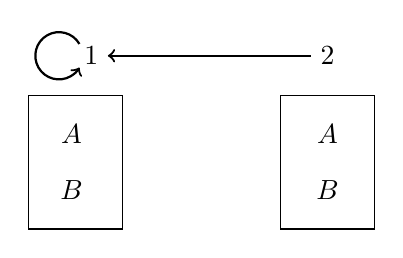
\begin{tikzpicture}
		\node (atom1) at (0,1) {1};
		\node (atom2) at (3,1) {2};
		\node (atom3) at (-0.25,0) {$A$};
		\node (atom4) at (3,0) {$\enot A$};
		\node (atom5) at (-0.25,-0.7) {$\enot B$};
		\node (atom6) at (3,-0.7) {$B$};
		\draw[->, thick] (atom1)+(-0.15,0.15) arc (-330:-30:.3);
		%\draw[->, thick] (atom2)+(0.15,-0.15) arc (-150:150:.3);
		\draw[<-, thick] (atom1) -- (atom2);
		\draw (-0.8,-1.2) rectangle (0.4,0.5);
		\draw (2.4,-1.2) rectangle (3.6,0.5);
	\end{tikzpicture}
	\end{arialabel}
\end{center}

下面是如何从图表中读出该解释的细节。它只包含两个世界，1 和 2。世界之间的箭头表示可及关系。所以 1 和 2 都可及 1，但 1 和 2 都不可及 2。每个世界旁边的方框让我们知道哪些原子语句在每个世界中为真：$A$ 在 1 中为真但在 2 中为假；$B$ 在 1 中为假但在 2 中为真。你只能在这些方框中写入一个原子语句或一个原子语句的否定。我们可以据此推算出更复杂的语句在每个世界中得到什么真值。例如，在这个解释下，以下所有语句在 $w_1$ 中都为真：
\[
A\eand\enot B,\qquad B\eif A,\qquad \ediamond A,\qquad \ebox\enot B
\]
如果你不喜欢用图示的方式思考，那么你也可以像这样呈现一个解释：

\begin{ekey}
	\item[W]$1,2$
	\item[R]$\langle 1,1\rangle, \langle 2,1\rangle$
	\item[\nu]$\nu_{1}(A)=T, \nu_{1}(B)=F, \nu_{2}(A)=F, \nu_{2}(B)=T$
\end{ekey}

稍后当我们开始考察\emph{反解释}时，你将有机会自己构造一些解释。

\section{系统 \mlK 的语义}
\label{SemanticsK}

现在我们可以将真值函项逻辑的所有语义概念扩展到模态逻辑：
\factoidbox{


\begin{factoiditems}
		\item $\metav{A}_1,\metav{A}_2, \dots
		\metav{A}_n\therefore\metav{C}$ 是\define{模态有效的（modally valid）}\ifeff{}
		在所有解释的所有世界中，不存在
		$\metav{A}_1,\metav{A}_2, \dots \metav{A}_n$ 全部为真而
		$\metav{C}$ 为假的情况。

		\item $\metav{A}$ 是\define{模态永真式（modal truth）}\ifeff{} $\metav{A}$
		在所有解释的所有世界中都为真。

		\item $\metav{A}$ 是\define{模态矛盾式（modal contradiction）}\ifeff{}
		$\metav{A}$ 在所有解释的所有世界中都为假。

		\item $\metav{A}$ 是\define{模态可满足的（modally satisfiable）}\ifeff{}
		$\metav{A}$ 在某个解释的某个世界中为真。
	\end{factoiditems}


		}
（从现在起，我们将省略明确的“模态”限定词，因为它们可以默认理解。）

我们也可以扩展 $\entails$ 的使用。但正如我们对 $\proves$ 所做的那样，我们需要再次添加下标。所以，当我们想表达 $\metav{A}_1,\metav{A}_2, \dots \metav{A}_n\therefore\metav{C}$ 有效时，我们将写作：$\metav{A}_1,\metav{A}_2, \dots \metav{A}_n\entails_\mlK\metav{C}$。

让我们通过给出一些反解释来更好地感受这种语义。考虑以下（错误的）主张：
\[\enot A\entails_\mlK \enot \ediamond A\]
为了给出这个主张的反解释，我们需要构造一个解释，使得 $\enot A$ 在某个世界 $w$ 上为真，而 $\enot\ediamond A$ 在 $w$ 上为假。这里有一个这样的解释，用图表表示如下：


\begin{center}
\begin{arialabel}{数字 1 和 2 由从 1 指向 2 的箭头连接。节点 1 标为 not-A，节点 2 标为 A。}
	\begin{tikzpicture}
		\node (atom1) at (0,1) {1};
		\node (atom2) at (3,1) {2};
		\node (atom3) at (-0.25,0) {$\enot A$};
		\node (atom4) at (3,0) {$A$};
		\draw[->, thick] (atom1) -- (atom2);
		\draw (-0.8,-0.6) rectangle (0.4,0.5);
		\draw (2.4,-0.6) rectangle (3.6,0.5);
	\end{tikzpicture}
\end{arialabel}
\end{center}


很容易看出，这将作为我们主张的反解释。首先，$\enot A$ 在世界 $1$ 上为真。其次，$\enot\ediamond A$ 在 $1$ 上为假：$A$ 在 $2$ 上为真，且 $2$ 可由 $1$ 可及。所以，在这个解释中存在某个世界，其中 $\enot A$ 为真而 $\enot\ediamond A$ 为假，因此并非 $\enot A\entails_\mlK\enot\ediamond A$。

为什么我们选择下标 \mlK？嗯，事实表明，系统 \mlK 与我们刚刚给出的有效性定义之间存在一个重要关系。具体来说，我们有以下两个结果：


\begin{compactlist}
	\item 如果 $\metav{A}_1,\metav{A}_2, \dots \metav{A}_n\proves_\mlK\metav{C}$，那么 $\metav{A}_1,\metav{A}_2, \dots \metav{A}_n\entails_\mlK\metav{C}$
	\item 如果 $\metav{A}_1,\metav{A}_2, \dots \metav{A}_n\entails_\mlK\metav{C}$，那么 $\metav{A}_1,\metav{A}_2, \dots \metav{A}_n\proves_\mlK\metav{C}$
\end{compactlist}


第一个结果被称为\emph{可靠性}结果，因为它告诉我们系统 \mlK 的规则是好的、可靠的规则：如果你能通过使用系统 \mlK 给出一个证明来证成一个论证，那么该论证确实是有效的。第二个结果被称为\emph{完备性}结果，因为它告诉我们系统 \mlK 的规则足够广泛，能捕捉所有有效论证：如果一个论证是有效的，那么就有可能用系统 \mlK 给出一个证明来证成它。

然而，陈述这些结果是一回事，证明它们又是另一回事。不过，我们不会在这里尝试证明它们。但可靠性证明背后的想法或许能让严格子证明的工作原理更清晰。

在严格子证明中，我们不能使用严格子证明之外的任何内容，除了我们使用 \ebox E 导入严格子证明的东西。如果我们已经假设或证明了 $\ebox \metav{A}$，那么通过 \ebox E，我们可以在严格子证明中使用 $\metav{A}$。而在系统 \mlK 中，这是将公式导入严格子证明的唯一方式。因此，在严格子证明内部所能证明的一切，都必须从在严格子证明外部我们有 $\ebox \metav{A}$ 的那些公式 $\metav{A}$ 推得。假设我们正在推理某个解释中一个可能世界上的真值。如果我们知道 $\ebox\metav{A}$ 在那个可能世界上为真，我们就知道 $\metav{A}$ 在所有可及世界上都为真。所以，在严格子证明内部所证明的一切在所有可及可能世界上都为真。这就是为什么 \ebox I 是一条可靠的规则。

\section{系统 \mlT 的语义}
\label{SemanticsT}

刚才我们说系统 \mlK 是可靠且完备的。那么我们考察过的其他模态系统，即系统 \mlT、\mlSfour 和 \mlSfive，情况又如何呢？嗯，相对于我们上面给出的有效性定义，它们都是\emph{不可靠的}。例如，所有这些系统都允许我们从 $\ebox A$ 推断 $A$，尽管 $\ebox A\nentails_\mlK A$。

这是否意味着这些系统毫无用处？完全不是！这些系统只是\emph{相对于我们上面给出的有效性定义}是不可靠的。（或者用符号来说，它们相对于 $\entails_\mlK$ 是不可靠的。）所以，当我们处理这些更强的模态系统时，我们只需要修改我们的有效性定义以适应。这正是可及关系真正派上用场的地方。

当我们引入可及关系这个概念时，我们说过它可以是任何你喜欢的世界之间的关系：你可以让它把每个世界与每个世界关联起来，不把任何世界与任何世界关联起来，或者介于两者之间。这就是我们在定义 $\entails_\mlK$ 时看待可及关系的方式。但如果我们愿意，我们可以开始对可及关系施加一些限制。特别是，我们可以坚持它必须是\emph{自反的}：
\[\forall w\, Rww\]
用自然语言说：每个世界都可及自身。或者用相对可能性来说：每个世界相对于自身都是可能的。如果我们施加这个限制，就可以引入一个新的后承关系 $\entails_\mlT$，定义如下：
\factoidbox{
	$\metav{A}_1,\metav{A}_2, \dots \metav{A}_n\entails_\mlT \metav{C}$ \ifeff{} 在任何\emph{具有自反可及关系的}解释中，都不存在一个世界，使得 $\metav{A}_1,\metav{A}_2, \dots \metav{A}_n$ 都为真而 $\metav{C}$ 为假
}
我们在 $\entails$ 上附加了 \mlT{} 下标，因为系统 \mlT{} 相对于这个新的有效性定义是可靠且完备的：


\begin{compactlist}
	\item 如果 $\metav{A}_1,\metav{A}_2, \dots \metav{A}_n\proves_\mlT\metav{C}$，那么 $\metav{A}_1,\metav{A}_2, \dots \metav{A}_n\entails_\mlT\metav{C}$
	\item 如果 $\metav{A}_1,\metav{A}_2, \dots \metav{A}_n\entails_\mlT\metav{C}$，那么 $\metav{A}_1,\metav{A}_2, \dots \metav{A}_n\proves_\mlT\metav{C}$
\end{compactlist}


和以前一样，我们不会试图证明这些可靠性和完备性结果。不过，相对容易看出，坚持可及关系必须是自反的将如何为 R\mlT{} 规则提供依据：
\factoidbox{


\begin{fitchproof}
			\have[m]{m}{\ebox \metav{A}}
			\have[\, ]{n}{\metav{A}}\rt{m}
	\end{fitchproof}


}
为了看清这一点，只需设想试图为以下断言构造一个反解释：
\[
	\ebox \metav{A}\entails_\mlT \metav{A}
\]
我们需要构造一个世界 $w$，使得在 $w$ 上 $\ebox \metav{A}$ 为真，而 $\metav{A}$ 为假。现在，如果 $\ebox \metav{A}$ 在 $w$ 上为真，那么 $\metav{A}$ 必须在 $w$ 所可及的每一个世界上为真。但由于可及关系是自反的，$w$ 可及 $w$。因此 $\metav{A}$ 必须在 $w$ 上为真。但现在 $\metav{A}$ 在 $w$ 上必定既\emph{为真}又\emph{为假}。矛盾！

\section{\mlSfour 的语义}
\label{SemanticsS4}

我们还可以如何调整有效性的定义？我们也可以规定可及关系必须是\emph{传递的}：
\[\forall w_1\forall w_2\forall w_3 ((Rw_1w_2 \eand Rw_2w_3)\eif Rw_1w_3)\]
用自然语言说：如果 $w_1$ 可及 $w_2$，且 $w_2$ 可及 $w_3$，那么 $w_1$ 可及 $w_3$。或者用相对可能性来说：如果 $w_3$ 相对于 $w_2$ 是可能的，且 $w_2$ 相对于 $w_1$ 是可能的，那么 $w_3$ 相对于 $w_1$ 就是可能的。如果我们在可及关系上加上这个限制，我们就可以引入一个新的后承关系 $\entails_\mlSfour$，定义如下：
\factoidbox{
	$\metav{A}_1,\metav{A}_2, \dots \metav{A}_n\entails_\mlSfour \metav{C}$ \ifeff{} 在任何\emph{具有自反且传递的可及关系的}解释中，都不存在一个世界，使得 $\metav{A}_1,\metav{A}_2, \dots \metav{A}_n$ 都为真而 $\metav{C}$ 为假
}
我们在 $\entails$ 上附加了 \mlSfour{} 下标，因为系统 \mlSfour{} 相对于这个新的有效性定义是可靠且完备的：


\begin{compactlist}
	\item 如果 $\metav{A}_1,\metav{A}_2, \dots \metav{A}_n\proves_\mlSfour\metav{C}$，那么 $\metav{A}_1,\metav{A}_2, \dots \metav{A}_n\entails_\mlSfour\metav{C}$
	\item 如果 $\metav{A}_1,\metav{A}_2, \dots \metav{A}_n\entails_\mlSfour\metav{C}$，那么 $\metav{A}_1,\metav{A}_2, \dots \metav{A}_n\proves_\mlSfour\metav{C}$
\end{compactlist}


和以前一样，我们不会试图证明这些可靠性和完备性结果。不过，相对容易看出，坚持可及关系必须是传递的将如何为 \mlSfour{} 规则提供依据：
\factoidbox{


\begin{fitchproof}
			\have[m]{m}{\ebox\metav{A}}
			\open
			\hypo[\ ]{k}{\ebox}\AS
			\have[\ ]{n}{\ebox\metav{A}}\rfour{m}
	\end{fitchproof}


}
请记住，严格子证明背后的思想是，它们是用来证明在所有可及世界中必然为真的事物的方法。所以 R$\mathbf{4}$ 规则意味着，每当 $\ebox \metav{A}$ 为真时，$\ebox \metav{A}$ 在每一个可及世界中也都必须为真。换句话说，我们必定有 $\ebox\metav{A} \entails_\mlSfour \ebox\ebox\metav{A}$。

为了看清这一点，只需设想试图为以下主张构造一个反解释：
\[\ebox\metav{A} \entails_\mlSfour \ebox \ebox \metav{A}\]
我们需要构造一个世界 $w_1$，使得在 $w_1$ 上 $\ebox\metav{A}$ 为真，而 $\ebox \ebox \metav{A}$ 为假。现在，如果 $\ebox \ebox \metav{A}$ 在 $w_1$ 上为假，那么 $w_1$ 必定可及某个世界 $w_2$，使得在 $w_2$ 上 $\ebox\metav{A}$ 为假。同样，如果 $\ebox \metav{A}$ 在 $w_2$ 上为假，那么 $w_2$ 必定可及某个世界 $w_3$，使得在 $w_3$ 上 $\metav{A}$ 为假。我们刚刚说过，$w_1$ 可及 $w_2$，且 $w_2$ 可及 $w_3$。因此，由于我们现在坚持可及关系是传递的，$w_1$ 必定可及 $w_3$。又因为 $\ebox\metav{A}$ 在 $w_1$ 上为真，且 $w_3$ 从 $w_1$ 可及，由此得出 $\metav{A}$ 在 $w_3$ 上必定为真。因此 $\metav{A}$ 在 $w_3$ 上既\emph{为真}又\emph{为假}。矛盾！

\section{\mlSfive 的语义}
\label{SemanticsS5}

让我们对可及关系再施加一个限制。这次，让我们坚持它也必须是\emph{对称的}：
\[\forall w_1\forall w_2(Rw_1w_2 \eif Rw_2w_1)\]
用自然语言说：如果 $w_1$ 可及 $w_2$，那么 $w_2$ 可及 $w_1$。或者用相对可能性来说：如果 $w_2$ 相对于 $w_1$ 是可能的，那么 $w_1$ 相对于 $w_2$ 也是可能的。逻辑学家将自反、对称且传递的关系称为\emph{等价关系}。我们现在可以定义一个新的后承关系 $\entails_\mlSfive $，如下所示：
\factoidbox{
	$\metav{A}_1,\metav{A}_2, \dots \metav{A}_n\entails_\mlSfive  \metav{C}$ \ifeff{} 在任何\emph{可及关系是等价关系的}解释中，都不存在一个世界，使得 $\metav{A}_1,\metav{A}_2, \dots \metav{A}_n$ 全部为真而 $\metav{C}$ 为假
}
我们在 $\entails$ 上附加了 \mlSfive{} 下标，因为系统 \mlSfive{} 相对于这个新的有效性定义是可靠且完备的：


\begin{compactlist}
	\item 如果 $\metav{A}_1,\metav{A}_2, \dots \metav{A}_n\proves_\mlSfive \metav{C}$，那么 $\metav{A}_1,\metav{A}_2, \dots \metav{A}_n\entails_\mlSfive \metav{C}$
	\item 如果 $\metav{A}_1,\metav{A}_2, \dots \metav{A}_n\entails_\mlSfive \metav{C}$，那么 $\metav{A}_1,\metav{A}_2, \dots \metav{A}_n\proves_\mlSfive \metav{C}$
\end{compactlist}


和之前一样，我们不会在这里尝试证明这些可靠性和完备性结果。不过，相对容易看出，坚持可及关系必须是等价关系将如何为 R$\mathbf{5}$ 规则提供依据：
\factoidbox{


\begin{fitchproof}
			\have[m]{m}{\enot\ebox \metav{A}}
			\open
			\hypo[\ ]{k}{\ebox}\AS
			\have[\, ]{n}{\enot\ebox\metav{A}}\rfive{m}
	\end{fitchproof}


}
该规则说的是，如果 $\metav{A}$ 并非必然，即在某个可及世界中为假，那么它在任何可及的可能世界中也都并非必然，也就是说，我们有 $\enot\ebox \metav{A} \proves_\mlSfive  \ebox\enot\ebox \metav{A}$。

为了看清这一点，只需设想试图为以下主张构造一个反解释：
\[
	\enot\ebox\metav{A} \entails_\mlSfive  \ebox \enot\ebox \metav{A}
\]
我们需要构造一个世界 $w_1$，使得在 $w_1$ 上 $\enot\ebox\metav{A}$ 为真，而 $\ebox \enot\ebox \metav{A}$ 为假。
现在，如果 $\enot\ebox\metav{A}$ 在 $w_1$ 上为真，那么 $w_1$ 必定可及某个世界 $w_2$，使得在 $w_2$ 上 $\metav{A}$ 为假。同样地，如果 $\ebox \enot\ebox \metav{A}$ 在 $w_1$ 上为假，那么 $w_1$ 必定可及某个世界 $w_3$，使得在 $w_3$ 上 $\enot\ebox \metav{A}$ 为假。既然我们现在坚持可及关系是一种等价关系，因而具有对称性，我们就可以推断 $w_3$ 可及 $w_1$。于是，$w_3$ 可及 $w_1$，且 $w_1$ 可及 $w_2$。再次利用我们现在坚持可及关系是一种等价关系（因而具有传递性）这一点，我们可以推断 $w_3$ 可及 $w_2$。但我们之前说过，在 $w_3$ 上 $\enot\ebox \metav{A}$ 为假，这意味着 $\metav{A}$ 在 $w_3$ 所可及的每一个世界上都为真。因此 $\metav{A}$ 在 $w_2$ 上既\emph{为真}又\emph{为假}。矛盾！

在 $\entails_\mlSfive $ 的定义中，我们规定可及关系必须是一个等价关系。但事实证明，还有另一种方法可以得到适合 \mlSfive 的有效性概念。我们不必规定可及关系是等价关系，而是可以规定它是一种\emph{全通}关系：
\[\forall w_1\forall w_2\, Rw_1w_2\]
用自然语言说：每个世界可及每个世界。或者用相对可能性来说：每个世界相对于每个世界都是可能的。使用这种对可及关系的限制，我们可以像下面这样定义 $\entails_\mlSfive $：
\factoidbox{
	$\metav{A}_1,\metav{A}_2, \dots \metav{A}_n\entails_\mlSfive  \metav{C}$ \ifeff{} 在任何\emph{具有全通可及关系}的解释中，都不存在一个世界，使得 $\metav{A}_1,\metav{A}_2, \dots \metav{A}_n$ 全部为真而 $\metav{C}$ 为假。
}
如果我们这样定义 $\entails_\mlSfive $，对于 \mlSfive 我们仍然会得到相同的可靠性和完备性结果。这告诉我们什么？嗯，这意味着，如果我们要处理的必然性概念认为\emph{每一个}世界都相对于\emph{每一个}世界是可能的，那么我们就应该使用 \mlSfive。更进一步，大多数哲学家都假定，他们最关心的那些必然性概念，比如\emph{逻辑必然性}和\emph{形而上学必然性}，恰恰就是这种类型。因此 \mlSfive{} 是大多数哲学家大多数时候使用的模态逻辑系统。

\practiceproblems

\problempart
给出下列错误主张的反解释：


\begin{compactlist}
	\item $\enot P \entails_\mlK \enot\ediamond P$
	\item $\ebox(P \eor Q)\entails_\mlK \ebox P \eor \ebox Q$
	\item $\entails_\mlK \enot \ebox (A\eand \enot A)$
	\item $\ebox A\entails_\mlK A$
\end{compactlist}

\problempart
给出下列错误主张的反解释：


\begin{compactlist}
	\item $\ediamond A\entails_\mlSfour \ebox\ediamond A$
	\item $\ediamond A, \ebox (\ediamond A \eif B)\entails_\mlSfour\ebox B$
\end{compactlist}

\problempart
给出下列错误主张的反解释：


\begin{compactlist}
	\item $\ebox (M\eif O),\ediamond M\entails_\mlT O$
	\item $\ebox A\entails_\mlT \ebox \ebox A$
\end{compactlist}

\section*{延伸阅读}

模态逻辑是逻辑学中一个庞大的子领域。我们仅仅触及了皮毛。如果你想了解更多关于模态逻辑的内容，可以参考以下教科书：

\begin{itemize}
	\item George E. Hughes 与 Max J. Cresswell 合著，《模态逻辑新导论》（\textit{A New Introduction to Modal Logic}），牛津：Routledge 出版社，1996年。
	\item Graham Priest 著，《非经典逻辑导论》（\textit{An Introduction to Non-Classical Logic}），第二版，剑桥：剑桥大学出版社，2008年。
	\item James W. Garson 著，《面向哲学家的模态逻辑》（\textit{Modal Logic for Philosophers}），第二版，剑桥：剑桥大学出版社，2013年。
\end{itemize}

这些作者都没有完全按照我们的方式来构建他们的模态证明系统，但最接近的构建方式是由 Garson 给出的。